\documentclass[a4paper, 12pt]{article}

\usepackage{a4wide}
\usepackage[utf8]{inputenc}
\usepackage[russian]{babel}
\usepackage[pdftex]{graphicx}
\usepackage{amsmath}
\usepackage{amssymb}
\usepackage{amsfonts}
\usepackage{graphicx}
\usepackage{hyperref}
\usepackage{verbatim}
\usepackage{indentfirst}
\usepackage[left=3cm, right=1.5cm, top=2cm, bottom=2cm]{geometry}
\setlength{\parindent}{1.25cm}
\linespread{1.3}
\setcounter{page}{2}

\newtheorem{myComment}{Замечание}
\newtheorem{myDef}{Определение}
\newtheorem{myProp}{Свойство}
\newtheorem{myTeor}{Теорема}
\newcommand{\dbtilde}[1]{\accentset{\approx}{#1}}
\DeclareMathOperator{\sign}{sign}

\begin{document}

\thispagestyle{empty}

\begin{center}
\vspace{-3cm}

\includegraphics[width=0.5\textwidth]{sources/msu.eps}\\
{\scshape Московский государственный университет имени}\\
М. В. Ломоносова\\
Факультет вычислительной математики и кибернетики\\
Кафедра суперкомпьютеров и квантовой информатики

\vfill

% {\LARGE }

\vspace{1cm}

{\Huge\bfseries Суперкомпьютерное моделирование и технологии}\\

\vspace{1cm}

{\LARGE Задание 2}
\end{center}

\vspace{1cm}

\begin{flushright}
  \large
  \textit{Студент 638 группы}\\
  М.\,И.~Хабибулин

  \vspace{5mm}

\end{flushright}

\vfill

\begin{center}
Москва, 2022
\end{center}

\newpage
\setcounter{tocdepth}{2}
\tableofcontents

\newpage
\normalsize

\section{Постановка задачи}

    Необходимо предоставить аналитическое решение и программную реализацию алгоритма численного решения задачи вычисления слудющего интеграла:
    
    \begin{equation}
        I = \int\int\limits_{G}\int {{(x^2 + y^2)}^{1/2}{dxdydz}},
    \end{equation}
    где область $G$ ограничена поверхностями $x^2 + y^2 = z^2$, $z = 1$.\\
    
    Также необходимо исследовать масштабируемость полученной программной реализации.
\section{Аналитическое решение}
\newpage
    \begin{figure}
    \centering
    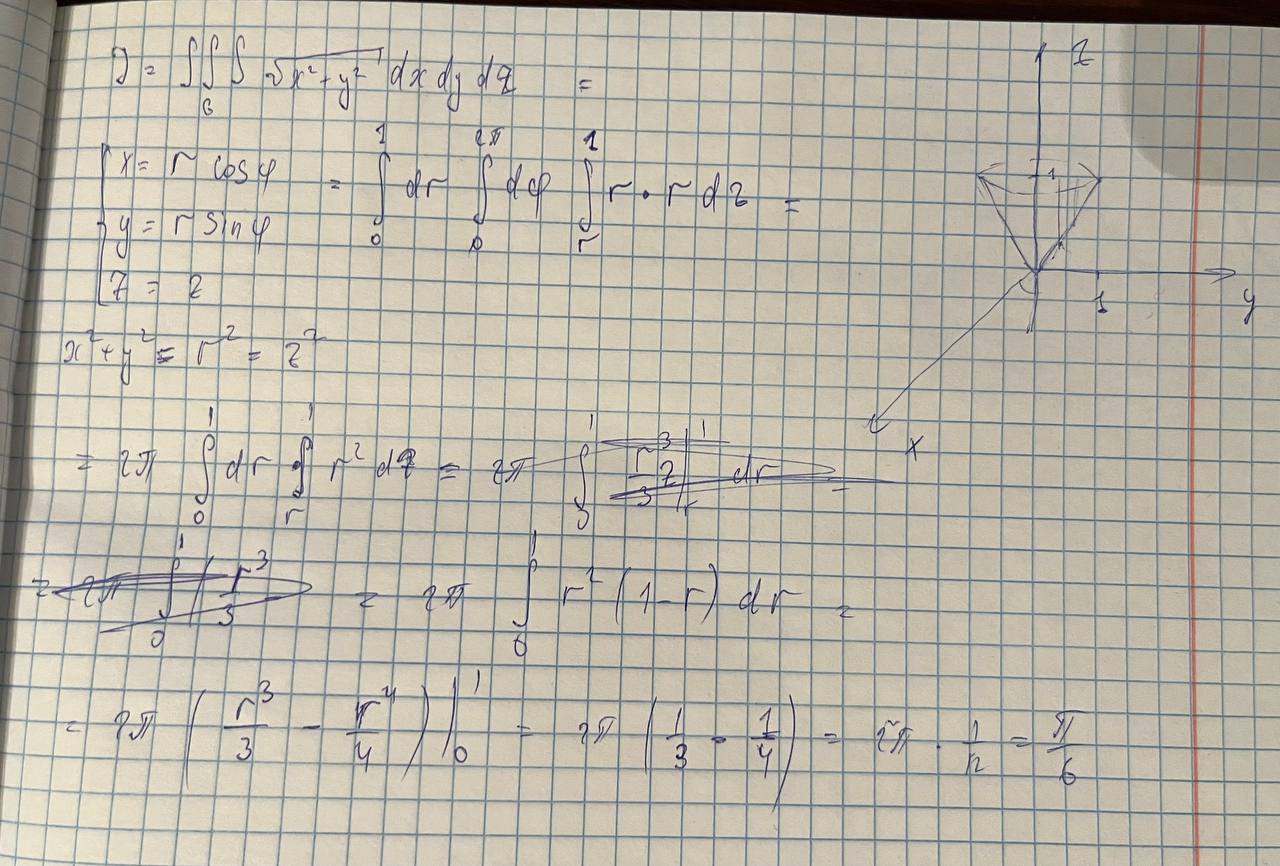
\includegraphics[width=1\textwidth]{1.jpg}
    \caption{\label{fig:frog}Аналитическое решение интеграла.}
    \end{figure}

    Таким образом, получаем аналитическое решение: $\frac{PI}{6}$.

\section{Описание численного алгоритма}

    Данная задача решается численно с использованием метода Монте-Карло: 
    \begin{enumerate}
        \item Задаем функцию $F(x, y, z)$ следующего вида:
            \begin{equation}
                F\left(x, y, z\right) = \left\{
                    \begin{array}{ll}
                        f\left(x, y, z\right) & \left(x, y, z\right) \in G, \\
                        0 & \left(x, y, z\right) \not\in G.
                    \end{array}
                \right.
            \end{equation}
        \item Далее преобразуем исходный интеграл:
            \begin{equation}
                I = \int\int\limits_{G}\int f\left(x, y, z\right)dxdydz = \int\int\limits_{G'}\int F\left(x, y, z\right) dxdydz.
            \end{equation}
            где $G'$ --- прямоугольник: $a_1 \leq x \leq b_1$, $a_2 \leq b_2$, $a_3 \leq b_3$.
        \item После этого семплируем случайные точки из $G'$ и на них считаем значение функции $F$.
        \item Окончательный результат получается из соотношения:
            \begin{equation}
                I' \approx \rvert G' \rvert \cdot \frac{1}{n} \sum\limits_{i = 1}^n F(p_i).
            \end{equation}
        \item Процесс продолжается до тех пор, пока значение ошибки не будет меньше некоторого наперед заданного значения $\varepsilon$: $|I - I'| < \varepsilon$.
    \end{enumerate}

\section{Результаты запуска программы}


\subsection{Polus}

    \begin{tabular}{|c|c|c|c|c|}
        \hline
        Точность $\varepsilon$ & Число MPI-процессов & Время работы (с) & Ускорение & Ошибка \\
        \hline
        3.0 \cdot 10^{-5} & 1 & 0.00206993 & 1 & 2.19904e-05\\
        3.0 \cdot 10^{-5} & 4 & 0.00115561 & 0.44 & 1.37322e-05\\
        3.0 \cdot 10^{-5} & 16 & 0.00075561 & 1.97 & 1.27422e-05\\
        3.0 \cdot 10^{-5} & 64 & - & - & -\\
        \hline
        5.0 \cdot 10^{-6} & 1 & 0.0036364 & 1 & 3.66476e-07\\
        5.0 \cdot 10^{-6} & 4 & 0.0016367 & 2.37 & 3.45779e-07\\
        5.0 \cdot 10^{-6} & 16 & 0.0012929 & 5.92 & 3.27479e-07\\
        5.0 \cdot 10^{-6} & 64 & - & - & -\\
        \hline
        1.5 \cdot 10^{-6} & 1 & 0.00461777 & 1 & 3.27479e-07\\
        1.5 \cdot 10^{-6} & 4 & 0.00283235 & 1.94 & 3.28379e-07\\
        1.5 \cdot 10^{-6} & 16 & 0.00197639 & 2.78 & 3.12478e-07\\
        1.5 \cdot 10^{-6} & 64 & - & - & -\\
        \hline
    \end{tabular}
    
    \begin{center}
        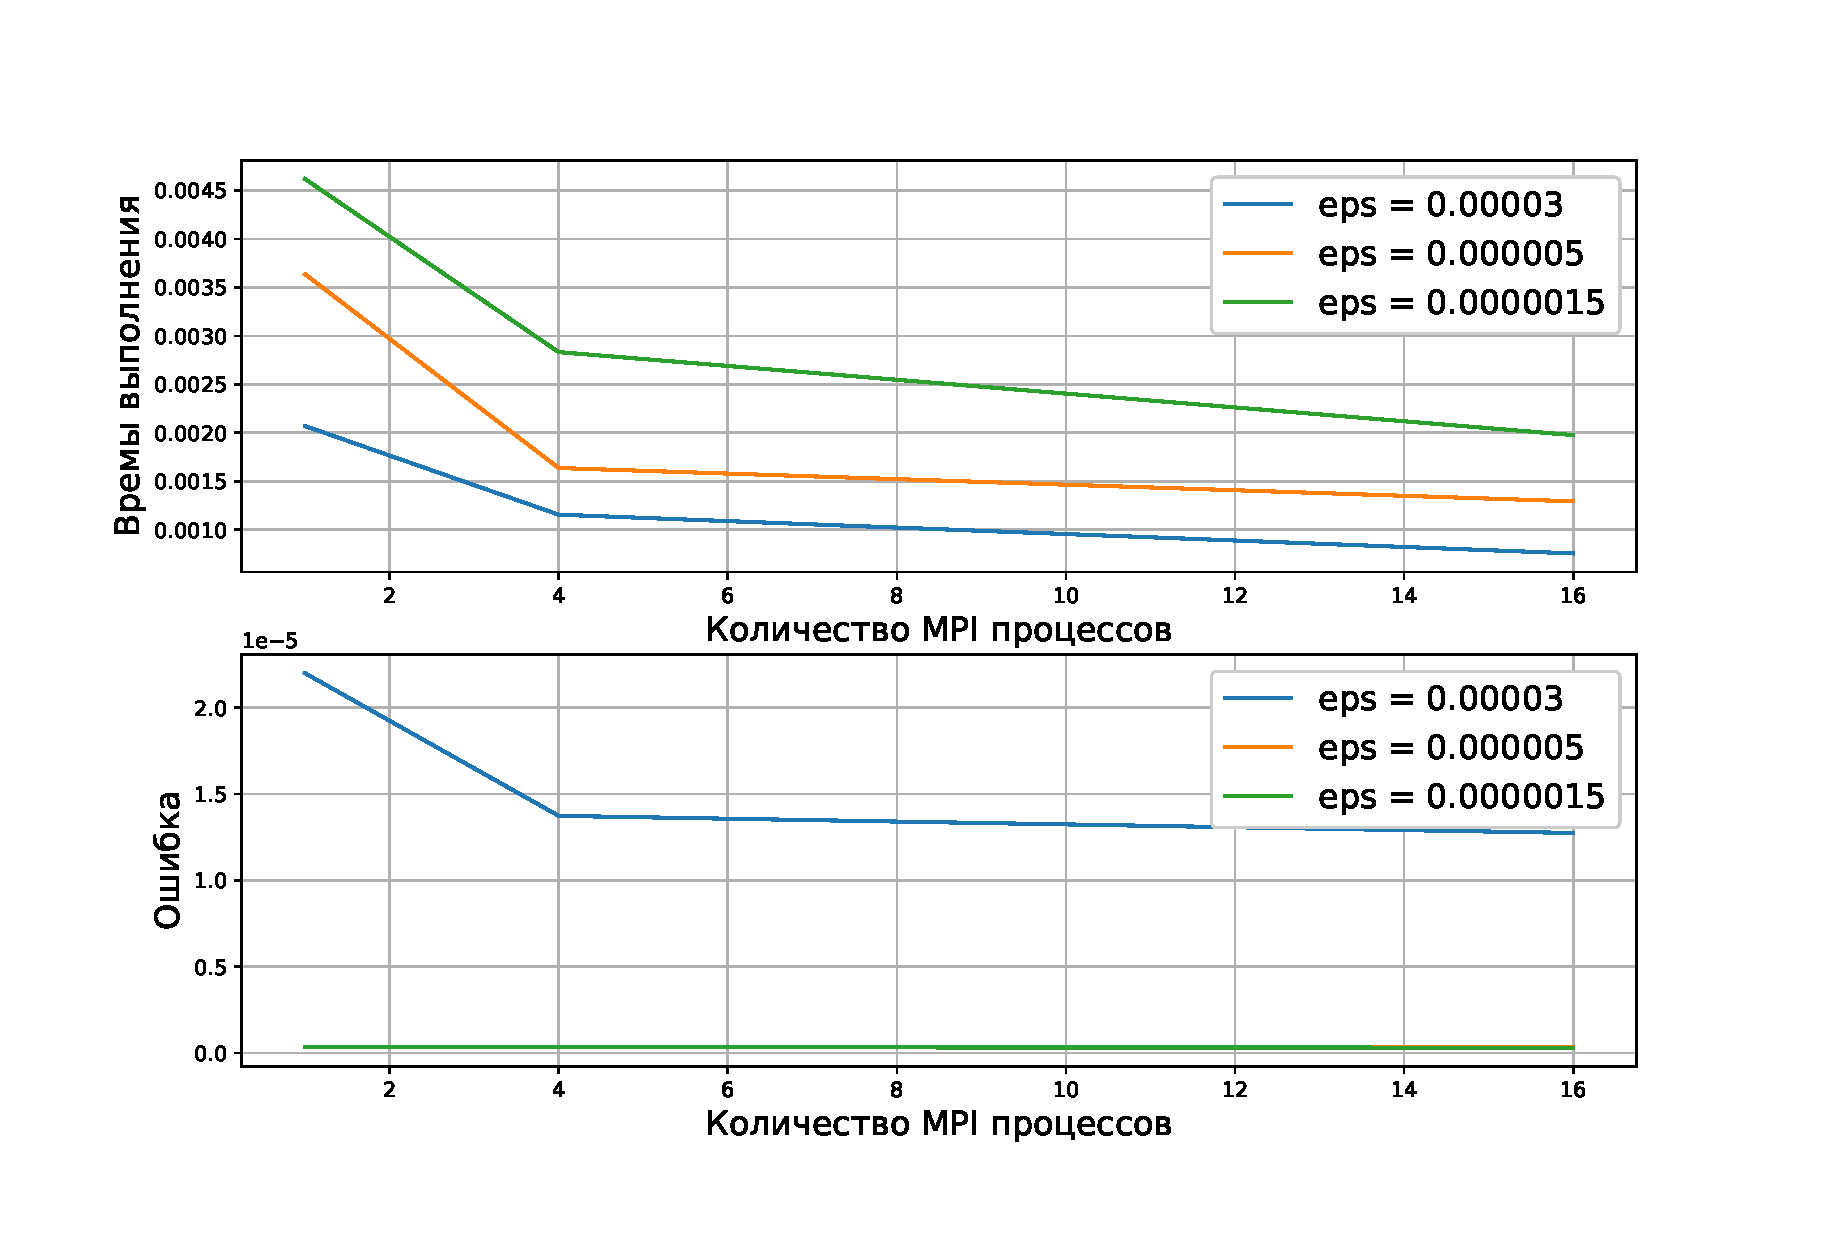
\includegraphics[width=0.8\textwidth]{sources/polus.eps}\\
        Рис. 2. Графики времени выполнения программы и ошибки на суперкомпьютере Polus в зависимости от количества процессов.
    \end{center}


\end{document}